\documentclass[a4paper, 11pt]{article}

\usepackage{amsmath} % Package for math
\usepackage{amssymb}
\usepackage{siunitx} % Provides the \SI{}{} command for typesetting SI units
\usepackage{graphicx} % Required for the inclusion of images
\usepackage{enumerate}
\usepackage{clrscode}
\usepackage{subfigure}
\usepackage{multirow}
\usepackage{dcolumn}

%\setlength\parindent{0pt} % Removes all indentation from paragraphs
\renewcommand\thesection{\Roman{section}}
\renewcommand\thesubsection{\roman{subsection}}
\renewcommand\thesubsubsection{\Alph{subsubsection}.}
\renewcommand{\End}{\kill\addtocounter{indent}{-1}\liprint\textbf{end} }
%\renewcommand{\labelenumi}{\alph{enumi}.} % Make numbering in the enumerate environment by letter rather than number (e.g. section 6)

\newtheorem{mydef}{Definition}
%\newtheorem{mydef}{Definition}

%\usepackage{times} % Uncomment to use the Times New Roman font

%----------------------------------------------------------------------------------------
%	DOCUMENT INFORMATION
%----------------------------------------------------------------------------------------

\title{The Application of\\ Multiobjective Evolutionary Algorithms\\ on Robot Path Planning System} % Title

\author{Wen \textsc{Li}} % Author name

\date{\today} % Date for the report

\begin{document}

\maketitle % Insert the title, author and date

\begin{center}
\begin{tabular}{l r}
%Date Performed: & October 18, 2013 \\ % Date the experiment was performed
Partners: & Wen Li \\ % Partner names
& Tu Yati\\
Instructor: & Professor Ying % Instructor/supervisor
\end{tabular}
\end{center}

% If you wish to include an abstract, uncomment the lines below
% \begin{abstract}
% Abstract text
% \end{abstract}

%----------------------------------------------------------------------------------------
%	ABSTRACT
%----------------------------------------------------------------------------------------
\begin{abstract}
\noindent This is a research report about \emph{Robot Path Planning} using \emph{Multiobjective Evolutionary Algorithm}(MOEAs)
and testing its feasibility and efficiency. In this article, we assigned three objectives to Robot the Planning problem.
Based on different preferences, decision makers require a set of solutions instead of one single result for their evaluation.
In this case, we adopt MOEAs, which is the core of whole system. Evolutionary algorithm has the characteristics to solve
\emph{the Multiobjective Optimization Problem}(MOP\cite{deb2001multi}): Firstly, it can produce more than one solution in each execution;
Second, by adding problem-specific heuristic methods, Pareto optimal solutions can be concluded.
So multiobjective evolutionary algorithms have been used to solve multiobjective optimization problems in recent years,
and have formed the different kinds of multiobjective evolutionary algorithms.\\
\\
This article adopts \emph{Non-dominated Sorting Genetic Algorithm II}(NSGA-II\cite{deb2000fast,deb2002fastelitist}),
\emph{Multiobjective Evolutionary Algorithm Based on Decomposition}(MOEA/D\cite{zhang2007moea}) and
\emph{Conical Area Evolutionary Algorithm}(CAEA\cite{weiqin2012efficient}), which are the core of the Robot Path Planning System.
We proposed three constraint conditions of path planning, which are Length, Smoothness and Security,
and established the mathematical modeling of MOP of the Robot Path Planning System.
For the specification of path planning, we adapted NSGA-II, MOEA/D and CAEA for they are suitable to solve this problem.\\
\\
\noindent \textbf{Keywords:} Path Planning, Multiobjective Optimization Problem, Evolutionary Algorithm, Pareto Optimal.
\newpage
\end{abstract}

%----------------------------------------------------------------------------------------
%   Contents
%----------------------------------------------------------------------------------------

\tableofcontents
\newpage
%----------------------------------------------------------------------------------------
%	INTRODUCTION
%----------------------------------------------------------------------------------------

\section{Introduction}
In this section, we will introduce the background and the value of the research project.\\
%----------------------------------------------------------------------------------------
%----------------------------------------------------------------------------------------
\subsection{Multiobjective Path Planning Overview}
%----------------------------------------------------------------------------------------
%----------------------------------------------------------------------------------------
\subsubsection{Background}
Path Planning is the act of finding a path to go from location A to B.
The purpose of Robot Path planning is to move the robot through an open field with obstacles in it.
In reality, path planning cares not only about Length, but also about some other criteria like Smoothness, Security and Energy Saving.
As a consequence, the path planning problem is actually a MOP and because of this, the solution of this problem would have
considerably realistic significance.\\
\\
In this article, we focus on three constraint conditions:
\begin{enumerate}[~~a.]
\item to find a path for robot from the start point to the destination ;
\item to make the path be secure for the robot;
\item to find the optimal path after first two conditions achieved;\newline
\end{enumerate}

%----------------------------------------------------------------------------------------
%----------------------------------------------------------------------------------------
\subsubsection{The Multiobjective Optimization Problem}
A multiobjective optimization problem can be stated as follows:
\begin{displaymath}
maximize \  F(x)=\big(f_1(x),\ldots,f_m(x)\big)^T
\end{displaymath}
\begin{equation}\label{eq:mop}
subject \  to \  x \in \Omega
\end{equation}
where $\Omega$ is the decision (variable) space, $F:\Omega\rightarrow R^m$ consists of $m$ real-valued objective functions
and $R^m$ is called the \emph{objective space}. The \emph{attainable objective} set is defined as the set $\{F(x)|x\in\Omega\}$.\\
\\
If $x\in R^n$, all the objectives are continuous and $\Omega$ is described by
\begin{displaymath}
\Omega=\{x\in R^n|h_j(x)\le 0, j=1,\ldots,m\}
\end{displaymath}
where $h_j$ are continuous functions, we call (\ref{eq:mop}) a \emph{continuous MOP}.\\
\\
As the objectives in (\ref{eq:mop}) contradict each other, there is no point in $\Omega$ that maximizes all the objectives simultaneously.
The best tradeoffs among them can be defined as Pareto optimality. \\
\\
Let $u, v\in R^m$, $u$ is said to dominate $v$ if and only if $u_i\ge v_i$ for every $i\in {1,\ldots,m}$ and $u_j>v_j$ for at least one index $j\in{1,\ldots,m}$.
A point $x^\ast \in\Omega$ is Pareto optimal to (\ref{eq:mop}) if there is no point $x\in\Omega$ such that $F(x)$ dominates $F(x^\ast)$.
$F(x^\ast)$ is then called a \emph{Pareto optimal (objective) vector}. In other words, any Pareto optimal point that improves in one objective
must lead deterioration in at least on other objective. The set of all the Pareto optimal points is called the \emph{Pareto Set}
(PS) and the set of all the Pareto optimal objective vectors is the \emph{Pareto front}(PF\cite{miettinen1999nonlinear}).

%----------------------------------------------------------------------------------------
%----------------------------------------------------------------------------------------
\subsection{Evolutionary Algorithm Overview}
In artificial intelligence, an \emph{evolutionary algorithm}(EA) is a generic population-based metaheuristic optimization algorithm.
An EA uses mechanisms inspired by \emph{biological evolution}, such as reproduction, mutation, recombination, and selection.
Candidate solutions to the optimization problem play the role of individuals in a population, and the evaluation function(or the fitness function)
determines the quality of the solutions. Evolution operations will be performed after the repeated execution of the above operators.
\emph{Genetic algorithms}(GA) belong to evolutionary algorithms.\\
\\
Some important terms of EAs have been as follows:
\begin{enumerate}[~~]
\item \textbf{Chromosome} also called \emph{a genome}, is a set of parameters which define a proposed solution to the problem
that EA is trying to solve;
\item \textbf{Individual} is an individual of chromosome;
\item \textbf{Population} is the set of all individuals;
\item \textbf{Fitness} is used as the indicator of the objective of an individual. The individual that has the better fitness has a higher rate to be selected for reproduction.
\item \textbf{Selection} is the stage of a EA in which individual are chosen from a population for later breeding (recombination or crossover).
\item \textbf{Crossover} is a genetic operator used to vary the programming of a chromosome or chromosomes from one generation to the next.
\item \textbf{Mutation} is a genetic operator used to maintain genetic diversity from one generation of a population of genetic algorithm chromosomes to the next.
\item \textbf{Fitness function} , also called \emph{Evaluation function}, is a particular type of objective function that is used to summarise how close a given design solution is to achieving the set aims.\\
\end{enumerate}
The pseudocode of EAs is as follow:

\begin{codebox}
\Procname{$\proc{Evolutionary Algorithm}$}
\li $\proc{ParameterInitialization()}$
\li \Comment Parameters like cross rate, mutation rate and generation number.
\li $\proc{PopulationInitialization(\id{population})}$
\li \For $i \gets 0$ \To $\id{gen\_num}$     \label{li:for}
\li \Comment or use other stopping criterion
\li     \Do                                  \label{li:for-begin}
\li     \While $j<\id{population\_size}$     \label{li:while}
\li         \Do $FitnessFunction(j)$       \label{li:while-begin}
\li             $j \gets j+1$             \label{li:while-end}
\li         \End
\li         $\id{parent\_idx} \gets \proc{SelectOperator()}$
\li         $\id{child\_idx} \gets \proc{CrossoverOperator(\id{parent\_idx})}$
\li         $\id{offspring} \cup \proc{MutationOperator(\id{child\_idx})}$
\li         $\id{population} \cup \id{offspring}$
\li         $i \gets i+1$          \label{li:for-end}
\li     \End
\end{codebox}
Brief Summarize:
\begin{enumerate}[1)]
\item In \emph{Select Operator}, only the individuals with relatively high fitness would be selected and reproduce offspring.
\item \emph{Crossover Operator} is priority to \emph{Mutation Operator}.
\item \emph{Cross rate} and \emph{Mutation rate} are the values in $(0.0, 1.0)$.
\item In this article, we assign fitness equal to the objective.
\end{enumerate}
%----------------------------------------------------------------------------------------
%----------------------------------------------------------------------------------------
\subsection{Section Conclusion}
In this section, we introduce the background of Robot Path Planning System,
and the overview of MOPs and EAs. Some of these are based on previous research
and on the next, we will concentrate on our new work about this problem.

\newpage
%----------------------------------------------------------------------------------------
%	Basics
%----------------------------------------------------------------------------------------
\section{Basics}
In this section, we will introduce the basics about NSGA-II, MOEA/D and CAEA,
and specify the mathematical model of the Robot Path Planning Problem.
\\
%----------------------------------------------------------------------------------------
%----------------------------------------------------------------------------------------
\subsection{NSGA-II Overview}
The NSGA-II is one of the most popular multi-objective EAs based on dominance, which is an improved version of NSGA\cite{}.
It sorts the individuals in the population by their dominance depths to keep the closeness to the PF.
In addition to this, NSGA-II prefers the individuals with larger crowding distances to preserve the diversity of distribution
along the PF. NSGA-II has two important features as follows:
\begin{enumerate}[1)]
\item using \emph{a fast nondominated sorting procedure} and \emph{an elitist-preserving approach};
\item preserving diversity among solutions of the nondominated solutions;
\end{enumerate}
Because of these two improvements, NSGA-II reduces the time-consuming from $O(MN^3)$ of NSGA to $O(MN^2)$.

\subsubsection{Fast Nondominated Sorting Approach}
Fast Nondominated sort, called FNDS for short, is the highlight part of whole algorithm.\\
\\
For each solution we calculate two entities: 1) domination count$n_p$, the number of solutions which dominate the
solution $p$, and 2)$S_p$, a set of solutions that the solution $p$  dominates. This requires $O(MN^2)$comparisons.\\
\\
Every solution in the first nondominated front will initialize their domination counter as zero.
Now, for each solution $p$ with $n_p=0$, we visit each member ($q$) of its set $S_p$ and reduce its domination count by one.
In doing so, if for any member $q$ the domination count becomes zero, we put it in a separate list $Q$. These
members belong to the second nondominated front. Now, the above procedure is continued with each member of $Q$ and the
third front is identified. This process continues until all fronts are identified.\\
\\
Following pseudocode is the procedure of the FNDS:
\begin{codebox}
\Procname{$\proc{FastNondominatedSort(\id{population})}$}
\li \For $p \in \id{population}$
\li     \Do
\li         $S_p \gets \emptyset$
\li         $n_p \gets 0$
\li         \For $\id{q} \in \id{population}$
\li             \Do
\li                 \If $(p \prec q)$               \label{fnds:if-p-q}
\li                 \Then
\li                       $S_p \gets S_p \cup \{q\}$ \label{fnds:Sp-q}
\li                 \Else \If $(q \prec p)$
\li                       \Then
\li                             $n_p \gets n_p+1$   \label{fnds:np_1}
                       \End
                    \End
\li               \End
\li         \If $(n_p = 0)$                     \label{fnds:np_0}
\li             \Then
\li                   $p_{rank} \gets 1$
\li                   $F_1 \gets F_1 \cup \{p\}$
\li             \End
\li    \End
\li $i \gets 1$                                 \label{fnds:init_fcntr}
\li \While $F_i \neq \emptyset$
\li     \Do
\li         $Q \gets \emptyset$                 \label{fnds:Q_empty}
\li         \For $p \in F_i$
\li             \Do
\li                 \For $q \in S_p$
\li                     \Do
\li                         $n_q \gets n_q-1$
\li                         \If $(n_q=0)$       \label{fnds:nq_0}
\li                             \Then
\li                                   $q_{rank}=i+1$
\li                                   $Q=Q\cup\{q\}$
                                \End
                        \End
\li             \End
\li         $i \gets i+1$
\li         $F_i=Q$
\li  \End
\end{codebox}
In the line \ref{fnds:if-p-q}, we can see that if $p$ dominates $q$, then $q$ will be added into the set of solutions dominated by $p$($S_p$). In the line \ref{fnds:np_0}, $p$ belongs to the first front if its counter is zero, and $p$ will have $p_{rank}=1$.

\subsubsection{Diversity Preservation}
NSGA-II uses the \emph{Crowding Distance Assignment}(CDA) to preserve diversity. $I[i].m$ stands for the objective $m$ of the idividual $i$.
The algorithm as shown at the below outlines the crowding-distance computation procedure of all solutions in an nondominated set $I$.

\begin{codebox}
\Procname{$CrowdingDistanceAssignment$}
\li $l=|I|$ \Comment number of solutions in $I$
\li \For $each\ i$
\li \Do
\li    $I[i]_{dist} \gets 0$
\li  \End
\li \For $each\ objective\ m$
\li     \Do
\li         $I=\proc{Sort(I, m)}$
\li         $I[1]_{dist} \gets I[l] \gets \infty$
\li         \For $i \gets 2\ to\ (l-1)$
\li           \Do
\li              $\mbox{\emph{diff}}\gets f^{max}_m - f^{min}_m$
\li              $I[i]_{dist} \gets I[i]_{dist}+(I[i+1].m-I[i-1].m)/\mbox{\emph{diff}}$
\li     \End
\end{codebox}

\subsubsection{Crowded-Comparison Operator}
The crowded-comparison operator ($\prec_n$) guides the selection process at the various stages of the algorithm. Assume that every individual $i$ in the population
has two attributes:
\begin{enumerate}[1)]
\item nondomination rank($i_{rank}$);
\item crowding distance($i_{dist}$);
\end{enumerate}
A partial order $\prec_n$ can be defined as:
\begin{displaymath}
i\prec_n j\quad\mbox{if}(i_{rank}<j_{rank})
\end{displaymath}
\begin{displaymath}
or\ ((i_{rank}=j_{rank})\ and\ (i_{dist}>i_{dist}))
\end{displaymath}

\subsubsection{Main Loop}
Now, this is the main process of the NSGA-II:
First, initialize the $P_0$ with a random function or a problem-specific function, and use $FNDS$ on every individual of the population. After that, do the evolution operators and then generate the offspring $Q_0$.
\begin{codebox}
\Procname{$NSGA-II$}
\li $R_t \gets P_t \cup Q_t$ \Comment combine parent and offspring population.
\li $F=\proc{FastNondominatedSort}(R_t)$
\li $P_{t+1}=\emptyset$and$i=1$
\li \Repeat \Comment repeat until the parent population is filled.
\li     $\proc{CrodingDistanceAssignment}(F_i)$
\li     $P_{t+1}=P_{t+1}\cup F_i$
\li     \Comment include $i$th nondominated front in the parent pop
\li     $i=i+1$
\li \Until $|P_{t+1}|+|F_i|\le N$
\li $\proc{Sort}(F_i,\prec_n)$ \Comment sort in descending order using $\prec_n$
\li $P_{t+1}=P_{t+1}\cup F_i[1:(N-|P_{t+1}|)]$
\li $Q_{t+1}=\proc{MakeNewPop}(P_{t+1})$
\li \Comment use selection, crossover and mutation to create a new population
\li $t=t+1$
\end{codebox}

%----------------------------------------------------------------------------------------
%----------------------------------------------------------------------------------------
\subsection{MOEA/D Overview}
Compared to NSGA-II, MOEA/D is a more efficient EA, which uses the decomposition strategy. \emph{Qingfu ZHANG} proposed this EA in 2007.

\subsubsection{Decomposition of Multiobjective Optimization}
There are several approaches for converting the problem of approximation of the PF into a number of scalar optimization problems.
In this article, we concentrate on one of them, which is Tchebycheff Approach\cite{miettinen1999nonlinear}.\\
\\
In Tchebycheff Approach, the scalar optimization problem is in the form
\begin{displaymath}
minimize g^{te}(x|\lambda, z^\ast)=\max_{1\le i\le m}\{\lambda_i|f_i(x)-z^\ast\}
\end{displaymath}
\begin{equation} \label{eq:tcheb}
subject\ to\ x\in\Omega
\end{equation}
where $z^\ast=(z^\ast_1,\ldots,z^\ast_m)^T$ is the reference point, i.e., if the goal is minimization, $z^\ast=\min\{f_i(x)|x\in\Omega\}$ for each $i=1,\ldots,m$.
For each Pareto optimal point $x^\ast$ there exists a weight vector $\lambda$ such that $x^\ast$ is the optimal solution of (\ref{eq:tcheb})
and each optimal solution of (\ref{eq:tcheb}) is a Pareto optimal solution of (\ref{eq:mop}). Thus, it is able to obtain different Pareto optimal solutions by altering the weight vector.

\subsubsection{The Framework of MOEA/D}
In the following description, the Tchebycheff approach is used as the decomposition method.\\
\\
Let $\lambda^1,\ldots,\lambda^N$ be a set of even spread weight vectors and $z^\ast$ be the reference point. By using the Tchebycheff approach the problem can be decomposed into $N$ scalar optimization subproblems, and the objective of the $j$th subproblem is
\begin{equation}\label{eq:gte}
g^{te}(x|\lambda^j, z^\ast)=\max_{1\le i\le m}\{\lambda^j_i|f_i(x)-z^\ast_i|\}
\end{equation}
where $\lambda^j=(\lambda^j_i,\ldots, \lambda^j_m)^T$. MOEA/D minimizes all these N objective functions simultaneously in a single run.\\
\\
In MOEA/D, a neighborhood of weight vector $\lambda^i$ is defined as a set of its several closest weight vectors in $\{\lambda_1,\ldots,\lambda_N\}$.
The neighborhood of the $i$th subproblem consists of all the subproblems with the weight vectors from the neighborhood of $\lambda^i$.
The population is composed of the best solution found so far for each subproblem.\\
\\
At each generation $t$, MOEA/D with the Tchebycheff approach maintains:
\begin{enumerate}[~~$\bullet$~~]
\item a population of $N$ points $x^1,\ldots,x^N\in\Omega$, where $x^i$ is the current solution to the $i$th subproblem;
\item $FV^1,\ldots,FV^N$, where $FV^i$ is the F-value of $x^i$, i.e., $FV^i=F(x^i)$ for each $i=1,\ldots,N$;
\item $z=(z_1,\ldots,z_m)^T$, where $z_i$ is the best value found so far for objective $f_i$;
\item an external population(EP), which is used to store nondominated solutions found during the search.
\end{enumerate}
The algorithm works as follows:\newline
\textbf{Input}:
\begin{enumerate}[~~$\bullet$~~]
\item MOP(1);
\item a stopping criterion;
\item N: the number of the subproblems considered in MOEA/D;
\item a uniform spread of N weight vectors: $\lambda^1,\ldots,\lambda^N$;
\item T: the number of the weight vectors in the neighborhood of each weight vector.
\end{enumerate}
\textbf{Output}: EP.
This is the pseudocode:
\begin{codebox}
\Procname {$MOEA/D$}
\li \Comment \textbf{Initialization}
\li EP$\gets \emptyset$
\li \proc{\textbf{ComputeDistance}}:
\li \Do Compute the Euclidean distances
\li     between any two weight vectors
\li \End
\li
\li \proc{\textbf{InitializeNeighborhood}}:
\li \Do For each $i=1,\ldots,N,\ set B(i)={i_1,\ldots,i_T},$
\li     where $\lambda^{i_1},\ldots,\lambda^{i_T}$ are the $T$ closest weight vectors to $\lambda^i$.
\li \End
\li
\li \proc{\textbf{InitializePopulation}}:
\li \Do by random or a problem-specific method.
\li \End
\li \proc{\textbf{InitializeReference}}:
\li \Do by a problem-specific method.
\li \End
\li
\li \Comment \textbf{Update}:
\li \Repeat
\li     \For $i\gets1\ to\ N$
\li       \Do
\li           \proc{\textbf{Reproduction}()}
\li           \proc{\textbf{Improvement}()}
\li           \proc{\textbf{UpdateReference}}:
\li           \Do For each $j=1,\ldots,m$, if $z_j<f_j(y')$,
\li           Then $z_j \gets f_j(y')$
\li           \End
\li
\li           \proc{\textbf{UpdateNeighborhood}}: \label{moead:neighbor}
\li           \Do For each index $j\in B(i)$,
\li           if $g^{te}(y'|\lambda^j,z)\le g^{te}(y^j|\lambda^j,z),$
\li           then set $x^i=y'$ and $F-value^j=F(y')$
\li           \End
\li           \proc{\textbf{UpdateEP}}:
\li           \Do Remove from EP all the vectors
\li               which are dominated by $F(y')$.
\li               If no vectors in EP dominate $F(y')$,
\li               add $F(y')$ to EP.
\li            \End
\li       \End
\li \Until $(\id{stop\_criteria}=true)$
\end{codebox}
We can see from the algorithm, the majority of time-consuming is updating $T$ neighborhood(line \ref{moead:neighbor}). Therefore, the time-consuming of MOEA/D is $O(NT)$. Because $T<N$, MOEA/D is more time-efficient than NSGA-II.
%----------------------------------------------------------------------------------------
%----------------------------------------------------------------------------------------
\subsection{CAEA Overview}
A \emph{Conical Area Evolutionary Algorithm} is proposed by \emph{Weiqin YING} to further improve computational efficiencies of evolutionary algorithms for bi-objective optimization. CAEA partitions the objective space into a number of conical subregions and then the MOP becomes a set of scalar optimization subproblem.

\subsubsection{Conical Partition Strategy}
It requires an \emph{utopia point} and a \emph{nadir point} in the objective space to partition the decision space.
Let $A$ be a set of solutions, $A\in\Omega$. The utopia point and the nadir point of A are respectively:
$F^\triangle(A)=(f^\triangle_1(A),f^\triangle_2(A))\textrm{ and } F^\nabla(A)=(f^\nabla_1(A),f^\nabla_2(A))$
where $f^\triangle_i(A)=\min\limits_{x\in A} f_i(x)\textrm{ and } f^\nabla_i(A)=\max\limits_{x\in A}f_i(x),i=1,2$
In addition, the transformed objective vectors are required: $\bar{y}=y-F^\triangle(A)$. After this transformation, the utopia point is at the origin$(0,0)$.

\begin{mydef}\emph{(Observation vector).}
The observation vector for any transformed point $\bar{y}=(\bar{y_1},\bar{y_2})$ is $\bar{V}(\bar{y})=(\bar{v_1}(\bar(y)),\bar{v_2}(\bar{y}))$ where $\bar{v_i}(\bar{y})=\frac{\bar{y_i}}{\bar{y_1}+\bar{y_2}},i=1,2$.
\end{mydef}
The observation vector has these features: $\bar{v_i}(\bar{y})\leq0$, and $\bar{v_1}(\bar{y})+\bar{v_2}(\bar{y})=1$. Given a prescribed number of divisions N, a series of uniformly distributed observation vectors $\bar{V^{(k)}}$ can be defined as $\bar{V^{(k)}}=(\frac{k}{N-1}, 1-\frac{k}{N-1}),k=0\ldots N-1$.

\begin{mydef}\label{def:conisub}\emph{(Conical subregion).}
For the central observation vector $\bar{V^{(k)}}=(\frac{k}{N-1},1-\frac{k}{N-1}),k=0\ldots N-1,$ the region $\bar{C}={\bar{y}=(\bar{y_1},\bar{y_2})|\bar{y_1}\geq0\wedge\bar{y_2}\geq0}$
can be devided into $N$ conical subregions: $\bar{C^{(k)}}={\bar{y}\in \bar{C}|\frac{k-0.5}{N-1}\le\bar{v_1}(\bar{y})<\frac{k+0.5}{N-1}}$,\\$k=0\ldots N-1$ where k is called the index of the sub region $\bar{C^{(k)}}$.
\end{mydef}
It can be inferred by Def.\ref{def:conisub} that the index of the subregion in which a solution $x\in A$ lies is $k= \llcorner\frac{(N-1)(f_1(x)-f^\triangle_1(A))}{f_1(x)-f^\triangle_1(A)+f_2(x)-f^\triangle_2(A)}+\frac{1}{2}\lrcorner$
where $\llcorner \cdot \lrcorner$ denotes the bottom integral function.

\subsubsection{Conical Area Indicator}
CAEA borrows the feature of \emph{hypervolume} to present an efficient conical area indicator for bi-objective area.

\begin{mydef}\emph{(Conical area).}
Let $\bar{y'}\in\bar{C^{(k)}}$, $0\le k\le N-1$, $\bar{y'}$ denote the reference point which should be an approximate infinity point dominated by all feasible solutions, then the conical area for $\bar{y'}$ is the area of the portion $\tilde{C}(\bar{y'})=\{\bar{y}\in\bar{C^{(k)}}|\neg(\bar{y'}\prec\bar{y})\wedge\bar{y}\wedge\bar{y'}\}$
, written as $S(\bar{y'})$.
\end{mydef}
The conical area $S(\bar{y'})$ is the sum of the area of two triangles conical area $\triangle OL^{(1)}U^{(1)}$ and $\triangle \bar{y'}U^{(2)}U^{(1)}$ where $U^{(1)}=(a\bar{y'_2},\bar{y'_2})$ is the intersection between $\bar{y_2}=\bar{y'_2}$ and the upper boundary of $\bar{C^{(k)}}$:
$$
S(\bar{y'})\ =\ 0.5(b-a)(\bar{y'_2})^2+0.5\frac{1}{a}(\bar{y'_1}-a\bar{y'_2})^2
$$
\begin{equation}
\quad\, =0.5\frac{1}{a}(\bar{y'^2_1})^2+0.5b(\bar{y'_1})^2-\bar{y'_1}\bar{y'_2}).
\end{equation}
However, it still requires some work to prove the connection between the conical area indicator and local Pareto optimality.
Because of the length of this report, the process of the proof will not be involved.
In conclusion, the indicator possesses the feature of local Pareto optimality,
so that the solution with the minimal conical area must be nondominated in the decision subset.

\subsubsection{Main Process of CAEA}
In CAEA, the $k$th scalar subproblem $g^{caea,k},0\le k\le N-1$, uses the conical area as its scalar objective in the form:
$$
minimize\ g^{caea,k}(x)=S(F(x)-F^\triangle(\Omega))
$$
\begin{equation}
subject\ to\ x\in\Omega^{(k)}.
\end{equation}
The $k$th individual in the population of CAEA is just the best solution $x^k$ found so far for the subproblem $g^{caea,k}$. Each generation of CAEA only produce one child $x'$. CAEA uses an area-based tournament selection \emph{AreaTour()} for the solutions with smaller conical areas should be preferred in the neighboring subregions. The pseudocode is as shown below:\\
\\
\emph{AreaTour()}
\begin{enumerate}[~~~1)]
\item Randomly select two indexes $a,\ b$ from $0\ldots N-1$.
\item Set $a_1\gets a-1$ and $a_2\gets a+1$. If $a=0$ then $a_1=2$ else if $a=N-1$ then $a_2=N-3$. Then $b_1$ and $b_2$ are set similarly in terms of $b$.
\item If ($\frac{S(F(x^{a_1}))+S(F(x^{a_2}-F^\triangle))}{2}-S(F(x^a)-F^\triangle)>$\\
$\quad\frac{S(F(x^{b_1}))+S(F(x^{b_2}-F^\triangle))}{2}-S(F(x^b)-F^\triangle)$) then $k\gets a$ else $k\gets b$
\item \textbf{Output}: $k$th index of the selected solution in $P$.
\end{enumerate}
CAEA only needs to update individual associated with the subproblem in terms of conical area in which the only offspring $x'$ lies. The whole algorithm works as follows:

\begin{codebox}
\Procname {\textbf{Step 1 Initialization}:}
\li \Do
\li \textbf{Generate} $N$ initial solutions $A\gets\{z^0,\ldots,z^{N-1}\}$
\li by randomly sampling from $\Omega$.
\li
\li \textbf{Initialize} $F^\triangle\gets(f^\triangle_1,f^\triangle_2)$ and $F^\nabla\gets(f^\nabla_1,f^\nabla_2)$
\li by setting $f^\triangle_i\gets\min_{0\le j\le N-1}f_i(z^j),\ f^\nabla_i\gets\max\limits_{0\le j\le N-1}f_i(z^j)$.
\li
\li \proc{\textbf{InitializePopulation}}:
\li Create a population $P\gets\{x^0,\ldots,x^{N-1}\}$
\li where $x^0=\ldots=x^{N-1}=null$.
\li Set $A'\gets A$.
\li
\li For each$k=0\ldots N-1$: if $A^{(k)}\neq\emptyset$,
\li then $x^k\gets\arg \min\limits_{z\in A^{(k)}}S(F(z)-F^\triangle)$ and $A'\gets A'-x^k$.
\li
\li For each $k=0\ldots N-1$: if $x^k=null$,
\li then $x^k\gets\arg \min\limits_{z\in A'}d(\bar{V}(F(z)-F^\triangle),\bar{V^{(k)}})$ \label{caea:step1d}
\li and $A'\gets A'-x^k$.
\li
\li Set $nE\gets N$ and $L\gets \ulcorner\frac{N}{10}\urcorner$.
\li \End
\end{codebox}

\begin{codebox}
\Procname {\textbf{Step 2 Evolution}:} \label{caea:step2}
\li \Do
\li     \proc{\textbf{Selection}}:
\li     Set $iL\gets nE\mod L$. \label{caea:step2mod}
\li     If $iL<2$, then $p_1\gets iL\times(N-1)$ else $p_1\gets AreaTour()$.
\li      Set $p_2\gets Areatour()$
\li
\li     \proc{\textbf{Reproduction}}:
\li     Create an offspring $x'$ from $x^{p_1}$ and $x^{p_2}$
\li     using genetic operators.
\li     Set $nE \gets nE+1$
\li
\li     \proc{\textbf{Update $F^\triangle$ and $F^\nabla$}}
\li     For each $i=1,2$, if $f_i(x')<f^\triangle_i$,
\li     then set $f^\triangle_i\gets f_i(x')$ and
\li     if $f_i(x')>f^\nabla_i$,
\li     then set $f^\nabla_i\gets f_i(x')$.
\li
\li     \proc{\textbf{Update $x^k$}}:
\li     Set $k_1\gets\llcorner\frac{(N-1)(f_1(x')-f^\triangle_1)}{f_1(x')-f^\triangle_1+f_2(x')-f^\triangle_2}+\frac{1}{2}\lrcorner$
\li     and $k_2\gets\llcorner\frac{(N-1)(f_1(x^{k_1})-f^\triangle_1)}{f_1(x^{k_1})-f^\triangle_1+f_2(x^{k_1})-f^\triangle_2}+\frac{1}{2}\lrcorner$
\li
\li     If $k_2\neq k_1\vee S(F(x')-F^\triangle)<S(F(x^{k_1}-F^\triangle))$
\li     then set $x^{k_1}\gets x'$
\li \End
\end{codebox}

\begin{codebox}
\Procname {\textbf{Step 3 Stoping Criterion}:}
\li \If the \emph{stopping criterion} is not satisfied
\li     \Then go back to \textbf{Step 2}
\li     \End
\end{codebox}

\begin{codebox}
\Procname {\textbf{Step 4 Post-processing}:}
\li \Do
\li     \textbf{Remove} the dominated solutions from
\li     the final population $P$ to obtain the approximate \emph{PS} $P'$.
\li
\li     \textbf{Output} $A'$ and the approximate \emph{PF} $F(P')$.
\li \End
\end{codebox}
where $\ulcorner\cdot\urcorner$ denotes the top integral function,
$d(\cdot,\cdot)$ represents the Euclidean distance between two vectors in \textbf{Step 1 line \ref{caea:step1d}} and $\mod$ in \textbf{Step 2 line \ref{caea:step2mod}} denotes the modulus operator.\\
\\
The major computational costs of CAEA are the update operations in \textbf{Step 2}. Since each child needs to update the individual of only one subproblems in \textbf{Step 2}, the complexity of CAEA is $O(1)$ for an offspring and $O(N)$ for $N$ offsprings. Hence CAEA has an extraordinary efficiency compared to NSGA-II($O(N^2)$) and MOEA/D($O(TN)$).

%----------------------------------------------------------------------------------------
%----------------------------------------------------------------------------------------
\subsection{Section Conclusion}
In this section, we made some introductions about three EAs which are used in this article. In the next section, the details of the algorithms will be presented.


\newpage
%----------------------------------------------------------------------------------------
%	Algorithm Design
%----------------------------------------------------------------------------------------

\section{Algorithm Design}
This section details the design of our experiment and algorithms. To transfer the \emph{Robot Path Planning} problem to a MOP, a specific math model is used and it will be presented on the next.\\
%----------------------------------------------------------------------------------------
%----------------------------------------------------------------------------------------
\subsection{Experimental Design}
As shown in the following figure, we can see that the start point and the destination point are fixed on the two corners on of the map. The size of this map is $20\times 20$. In the experiment, all the individuals are initialized randomly and optimized with EAs.
\begin{figure}[htb]
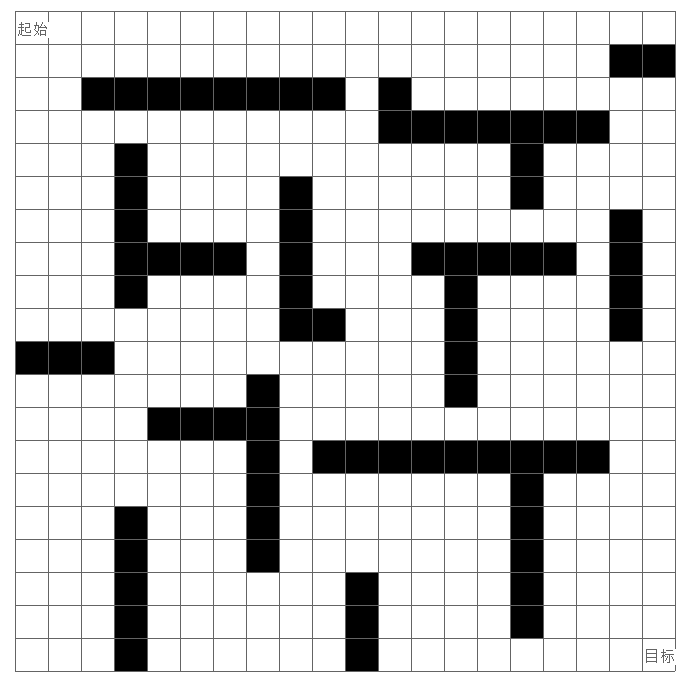
\includegraphics[width=0.9\textwidth]{images/20131122155512.png}
\caption{a sample path map}
\label{fig:path}
\end{figure}
This experiment is based on a random static environment, which means the blocks on the map are certain when the test begins and all the initializations are random. This environment has some features:

\begin{enumerate}[~~1)~]
\item Before the test starts, the position and the number of blocks can be modified.
    Other parameters like \emph{crossover rate}, \emph{mutation rate} and number of \emph{population} and \emph{generation} also are changeable.
\item During the test is running, all these parameters above can not be changed or modified.
\end{enumerate}

%----------------------------------------------------------------------------------------
%----------------------------------------------------------------------------------------
\subsection{Mathematical Model}
%----------------------------------------------------------------------------------------
\subsubsection{Code Chromosome}
To code \emph{chromosome}, this article employed \emph{vector} in \emph{C++ STL}. Each \emph{vector} stores one \emph{path} of an individual. Its structure:
$$
path\ =\ \{(x_0,y_0),(x_1,y_1),\ldots,(x_{n-1},y_{n-1})\}
$$
where $n$ is changeable. $(x_0,y_0)$ and $(x_{n-1},y_{n-1})$ stand for the start point and the destination point.
$(x_i,y_i),\, i=1,2,\ldots,n-2$ stand for the coordinates of the points on the map.\\
\\
An individual has the structure as follows:
$$
indiv\ =\ \{path,obj\}
$$
where \emph{indiv} is the initial of the individual and \emph{obj} stands for the vector of the objective values which acquire from \emph{objective function}. So we can conclude that the population is as shown below:
$$
population\ =\ \{indiv_1,indiv_2,\ldots,indiv_k\}\\
$$
$$
k=population size
$$
\subsubsection{Objective Function\cite{zhou2011multiobjective}}
First of all, task of path planning is to find a way from the start point to the destination point without blocked. Besides, this article assigned another three objectives: \emph{Length}, \emph{Smoothness} and \emph{Security}.\\
\\
The objective functions evaluate every path in every individual.
These are the main process:\\
\\
\textbf{~~a.~Length}
$$
F_1(P)=1-shortest\_len\big/\sum^{n-1}_{i=1}|p_i p_{i+1}|
$$
where \emph{shortest\_len} is the straight-line distance from the start point to the destination point. $|p_i p_{i+1}|$ is the distance of $p_i p_{i+1}$. This $F_1(P)$ is the objective function of \emph{Length} and the smaller $F_1(P)$ means the shorter \emph{Length}.\\
\\
\textbf{~~b.~Smoothness}\\
The \emph{Smoothness} uses the angle the path travelling as an indicator.
$$
\If\ n>2,\quad F_2(P)=\big((\sum^{n-1}_{i=2}\theta_i+k\frac{\pi}{2})/(n-2)\big)/\pi
$$
$$
\theta\ =\ \arccos\big(\frac{p_{i-1}p_i\cdot p_i p_{i+1}}{|p_{i-1}p_i||p_i p_{i+1}|}\big)
$$
$$
\If\ n=2,\quad F_2(P)=1.
$$
where, $\theta_i\ (i=2,\ldots,n-1)$ is the angle between $p_{i-1}p_i$ and $p_i p_{i+1}$. $k$ is the number of $\theta_i>\pi/2$, which means punishment. $F_2(P)$ is proportional to the average angle which the path $P$ travelled. As we can see from the above, the smaller $F_2(P)$ means the better smoothness.\\
\\
\textbf{~~c.~Security}\\
Since our robot is not a particle, \emph{Security} becomes a very important indicator. \emph{Security} is related to the distance between our moving object and blocks. The moving object should keep a secure distance to the block in case of the crashing.
$$
F_3(P)\ =\ 1-\big(average\_dist(p_n)-M\cdot imp\big)\ \big/\ (shortest\_len/2)
$$
$$
average\_dist(p_n)\ =\ \sum^{n-1}_{x=1}\big(\sum^{m}_{y=1}dis(x,y)\big)\ \big/\ (m\cdot n)
$$
where $average\_dist(p_n)$ is the function to calculate the average distance of every point in the $p_n$ to all blocks. $shortest\_len/2$ means the longest distance from the point to a block. $n$ is the number of points in the $n$th path $p_n$, while $m$ is the number of the blocks in the field. $M$ is a counter of the point of intersection of the path and the block. $M\cdot imp$ means the punishment for the intersection and in this article, $imp$ equals the width of the map.\\
\\
$F_3(P)$ is the objective function to evaluate the $Security$. The same as $Length$ and $Smoothness$, the lower the $Security$ is, the better.\\
\\
All these three objective functions have the domain of $[0,\ 1]$. Usually, the ideal value is $0$ which can not obtain.
In addition, it still requires an objective function to check whether the path passed the blocks or not.
We assigned a counter $D$ to record the number of blocks on the path, which is used as an indicator for punishment.
If $D$ of an individual is very big, it will be less possible to be selected to reproduce offspring.
This process is very simple, so that it will not be presented in this article.

\subsection{Evolution Operator}
Evolution operators play the important roles in reproduction.
In this article, we employed three evolution operators: \emph{Selection},
\emph{Crossover} and \emph{Mutation}. Operation of \emph{Selection} is related to
the implementation of each EA. As a consequence, this section will not introduce this again. In the following, we will concentrate on \emph{Crossover} and \emph{Mutation} operators.

\subsubsection{Crossover Operator}
If two paths have at least one same point, they can be crossed through the crossover operator. This operation requires two paths $path_1$ and $path_2$ from the parents, and then generates two children with paths related to both parents. There are two kinds of crossover, one is \emph{uniform crossover} and the other one is \emph{single-point crossover}. Based on the situation of this path planning problem, we decided to use single-point crossover. As the figure shown below:
\begin{figure}[htb]
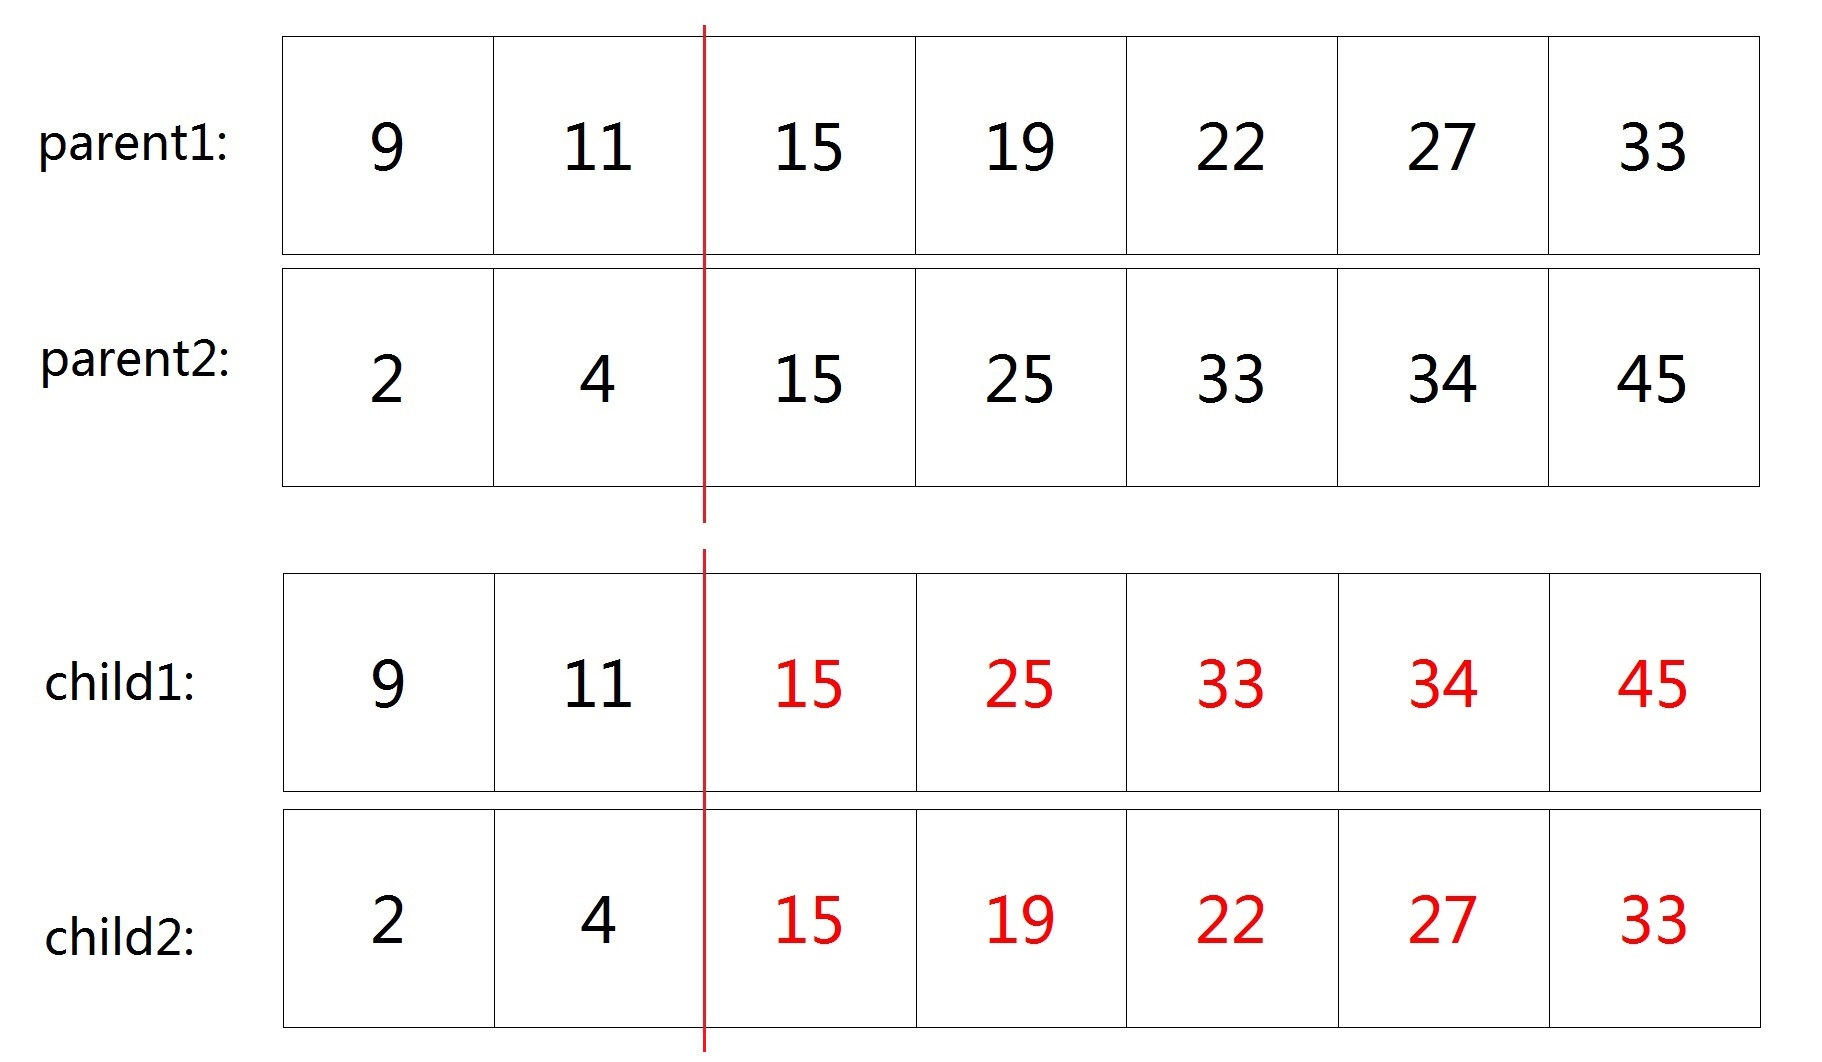
\includegraphics[width=0.9\textwidth]{images/crossover.jpg}
\caption{single-point crossover}
\label{fig:crossover}
\end{figure}
\\
Here is the pseudocode of crossover function:
\begin{codebox}
\Procname {$Crossover()$}
\li \textbf{Input:} $parent1$, $parent2$
\li Initialize $child1$ and $child2$
\li $r \gets \proc{Random()}$ in $[0.0,1.0]$
\li \If ($r<cross\_rate$)
\li     \Then random initialize $cross\_point$ in $parent1$ and $parent2$
\li           \For $i\gets 0$ to $cross\_point$
\li            \Do $child1_i\gets parent1_i$
\li                $child2_i\gets parent2_i$
\li            \End
\li           \For $j\gets cross\_point$ to $n-1$
\li            \Do $child1_j\gets parent1_j$
\li            \End
\li           \For $k\gets cross\_point$ to $n-1$
\li            \Do $child2_k\gets parent2_k$
\li            \End
\li     \Else   $child1\gets parent1$
\li             $child2\gets parent2$
\li \End
\li \textbf{Output:} $child1$, $child2$
\end{codebox}

\subsubsection{Mutation Operator}
Mutation operator plays the role of keeping the population diversity. The operation of mutation is not always heading the good way. on one hand, mutation operator can optimize the path in many situations, on the other hand, if this path is already feasible, mutation might damage this feasibility. %Because of this, this mutation operator include two different operations:
%\begin{enumerate}[~~1)~]
%\item If the path is feasible after the mutation, the operation is done.
%\item If the path is not feasible after the mutation, mutation failed and nothing has changed.
%\end{enumerate}
This is the pseudocode:
\begin{codebox}
\Procname {Mutation()}
\li \textbf{Input:} $population$
\li $indiv\in population$
\li \For $i\gets 0$ to $population\_size$
\li     \Do $r\gets \proc{Random()} $ in $[0.0,1.0]$
\li         \If ($r<mutation\_rate\And indiv_i\_size> 2$)
\li             \Then $point\gets \proc{Random()}$
\li                 \If ($\proc{isSeries}(point)\And
\proc{isBlock}(point)=false$) \label{mut:if}
\li                     \Then $point$ replace the point in $indiv_i$
\li                     \End
\li             \End
\li    \End
\li \textbf{Output}: $population$
\end{codebox}
where at line \ref{mut:if}, the mutation will be executed, only if $point$ is series to the next and the previous point of it and $point$ is not block point.

\subsubsection{Delete Operator}
\emph{Delete Operator} is a problem-specific operator. The function of this \emph{Delete} is to reduce the length of the path by deleting repetitions and the useless. This operator can speed up the whole algorithm. The following is the process of delete operator:
\begin{codebox}
\Procname {$Delete()$}
\li \textbf{Input}: $population$
\li $indiv\in population$
\li \For $i\gets 0$ to $population\_size-1$
\li \Do \For $j\gets 0$ to $indiv_i\_size$
\li         \Do \For $k\gets indiv_i\_size-1$ to $j$
\li             \Do \If ($k=j$)
\li                 \Then $point\gets k$
\li                       $flag\gets true$
\li                 \End
\li             \End
\li             \If $flag=true$
\li             \Then $delete\ indiv_{j\to k}$
\li             \End
\li         \End
\li \End
\li \textbf{Output}:$population$
\end{codebox}
%----------------------------------------------------------------------------------------
%----------------------------------------------------------------------------------------
\subsection{Section Conclusion}
In this section, we introduced the math model of \emph{Robot Path Planning} problem including, chromosome coding, parameter setting and objective functions. In addition, we presented three evolution operators employed in this article.


\newpage
%----------------------------------------------------------------------------------------
%	Environment and Configuration
%----------------------------------------------------------------------------------------

\section{Results and Analysis}

%----------------------------------------------------------------------------------------
%----------------------------------------------------------------------------------------
\subsection{Introduction to Experiment}
The experiment of \emph{Robot Path Planning} is based on the program we developed, so that we need to describe the features of this program.
\begin{enumerate}[~~1)~]
\item Three indicators, \emph{Length}, \emph{Smoothness} and \emph{Security}, have the same codomain $[0.000,\ 1.000]$. The lower the indicator becomes, the shorter, the smoother or the securer the path is.
\item The greater crossover rate leads to the faster convergence of Pareto solution set while the mutation rate is the opposite.
    The value of the mutation rate is dependent on other parameters. As an instance, the bigger the population is, the lower the mutation rate should be. In general, the crossover rate is in $[0.4,\ 0.9]$ and the mutation rate should be in $[0.001,\ 0.1]$.
\item This experiment employs a random static environment. The size of maps does not affect the value of parameters, like crossover rate, mutation rate, population size and total generation. Because of that, we decided to use a $20\times 20$ map as shown below:
\end{enumerate}
\begin{figure}[htb]
\centerline{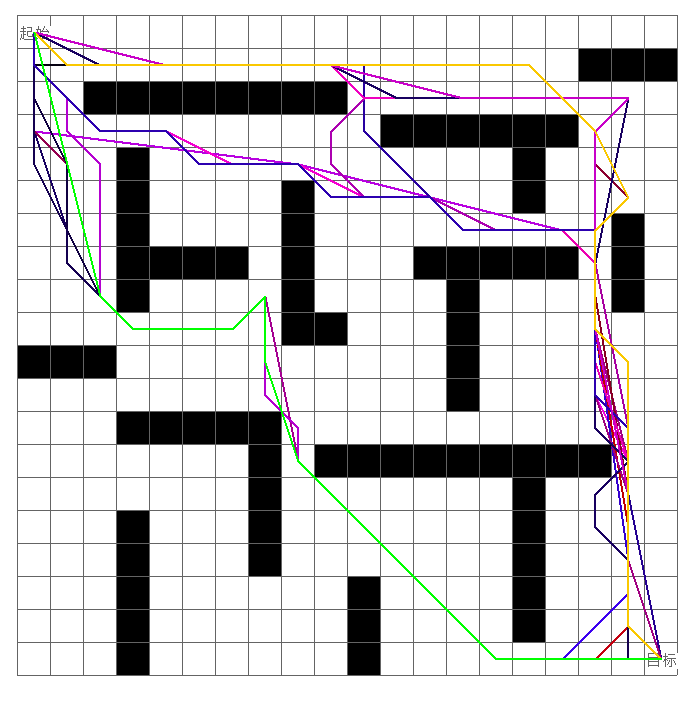
\includegraphics[width=0.7\textwidth]{images/2020.png}}
\caption{a running sample}
\end{figure}
%----------------------------------------------------------------------------------------
%----------------------------------------------------------------------------------------
\subsection{Data and Analysis}

\subsubsection{Test 1: Generations}
In this test, the parameters are as follows: $crossover\ rate\ =\ 0.9$;
$mutation\ rate\ =\ 0.1$; $population\ size\ =\ 100$. The variable is $generation$ from $100th$ to $500th$. These are the data of test 1:\\
\begin{table}[!htb]
  \centering
    \begin{tabular}{|l|l|c|c|c|c|c|}
    \hline
    \multicolumn{2}{|c|}{Generation:}& 100th & 200th & 300th & 400th & 500th\\
    \hline
    \multirow{3}{*}{NSGA-II}& Length & 0.365 & 0.356 & 0.328 & 0.360 & 0.286\\
                            & Smoothness & 0.708 & 0.100 & 0.143 & 0.143 & 0.143\\
                            & Security & 0.384 & 0.402 & 0.361 & 0.354 & 0.399\\
    \hline
    \multirow{3}{*}{MOEA/D} & Length & 0.374 & 0.378 & 0.373 & 0.344 & 0.370\\
                            & Smoothness & 0.186 & 0.114 & 0.146 & 0.151 & 0.140\\
                            & Security & 0.369 & 0.374 & 0.359 & 0.346 & 0.351\\
    \hline
    \multirow{3}{*}{CAEA}   & Length & 0.361 & 0.351 & 0.349 & 0.351 & 0.351\\
                            & Smoothness & 0.219 & 0.172 & 0.175 & 0.161 & 0.151\\
                            & Security & 0.382 & 0.341 & 0.343 & 0.344 & 0.344\\
    \hline
    \end{tabular}
  \caption{Data from 100th to 500th generation.}\label{tb:15}
\end{table}
\\
We can see from the table that the convergence of NSGA-II began at about $200th$ to $300th$ generation.
About MOEA/D, which is very similar to NSGA-II, also began to converge since around $300th$, while CAEA had
not converged too early for we can see the optimizing at $300th$, $400th$ and $500th$.
These are the running screenshots of three algorithms(green line is for the shortest path,
yellow one is for the smoothest and the purple line is for the securest line):\\
\begin{figure}[htb]
    \begin{center}
    \subfigure[NSGA-II]
    {
        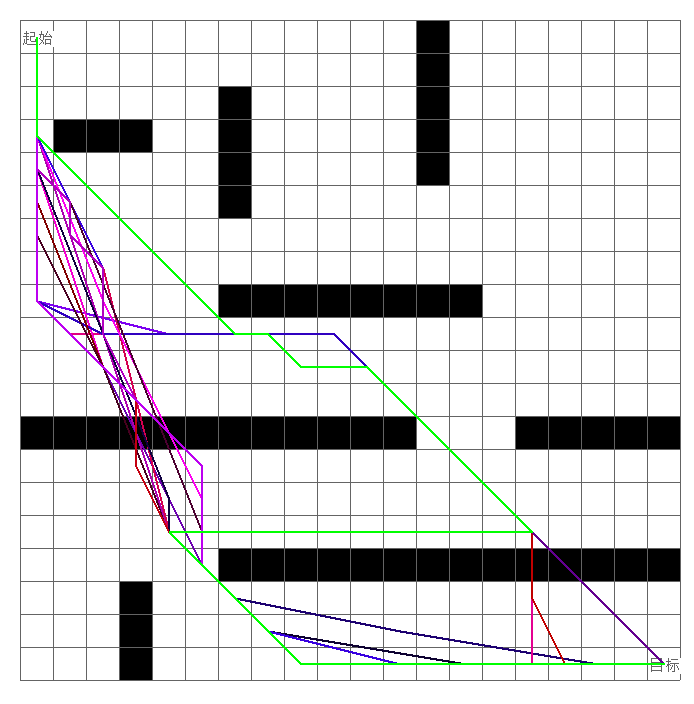
\includegraphics[width=1.5in]{images/100nsga.png}
    }
    \subfigure[MOEA/D]
    {
        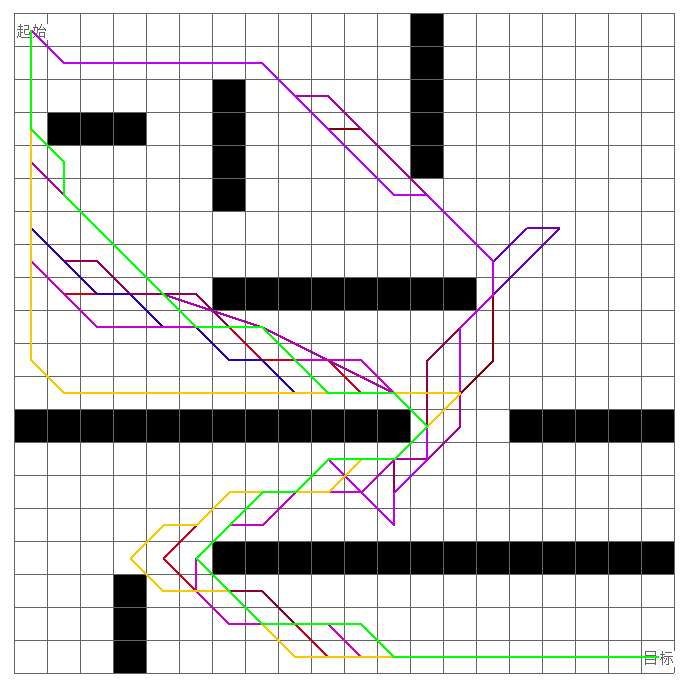
\includegraphics[width=1.5in]{images/100moead.png}
    }
    \subfigure[CAEA]
    {
        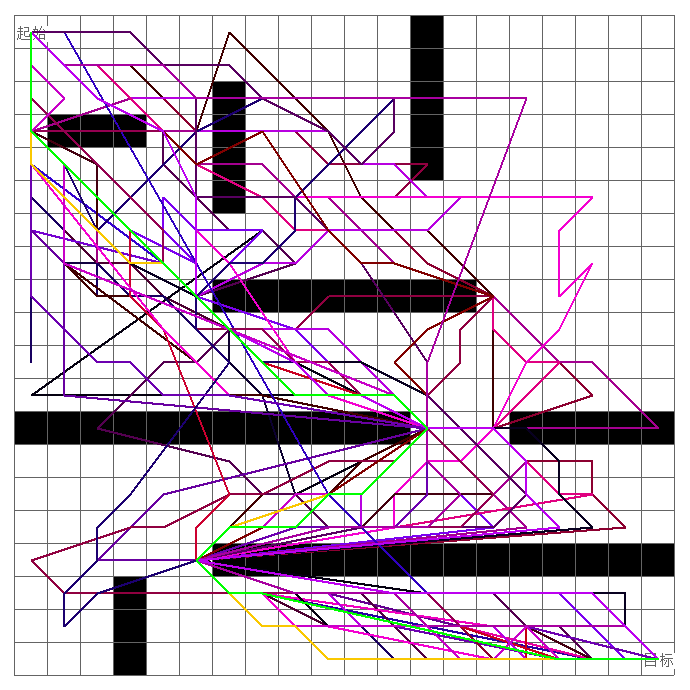
\includegraphics[width=1.5in]{images/100caea.png}
    }
    \end{center}
    \caption{Running screenshots at the $100th$}
\end{figure}
\newpage
\begin{figure}[htb]
    \begin{center}
    \subfigure[NSGA-II]
    {
        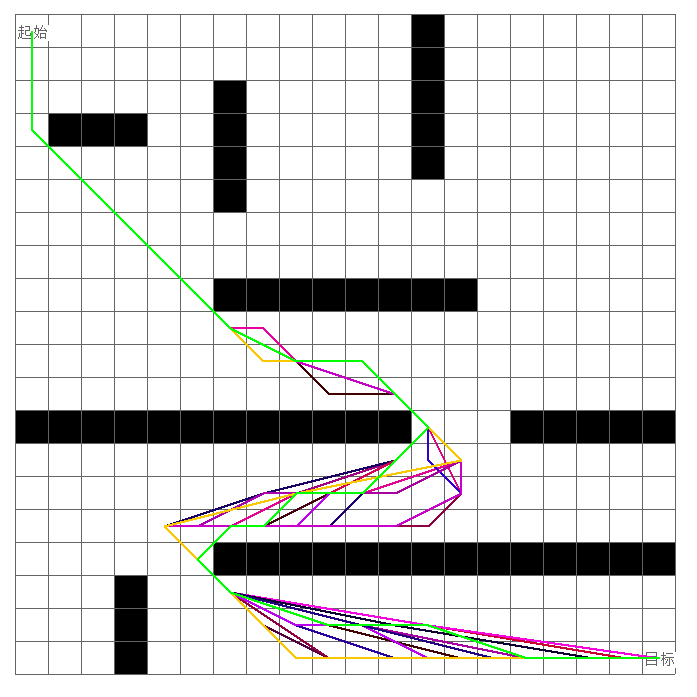
\includegraphics[width=1.5in]{images/200nsga.png}
    }
    \subfigure[MOEA/D]
    {
        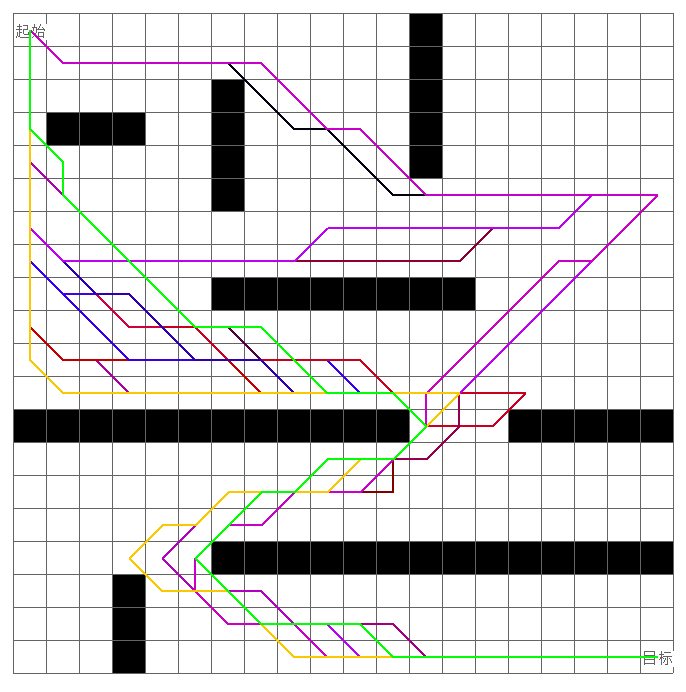
\includegraphics[width=1.5in]{images/200moead.png}
    }
    \subfigure[CAEA]
    {
        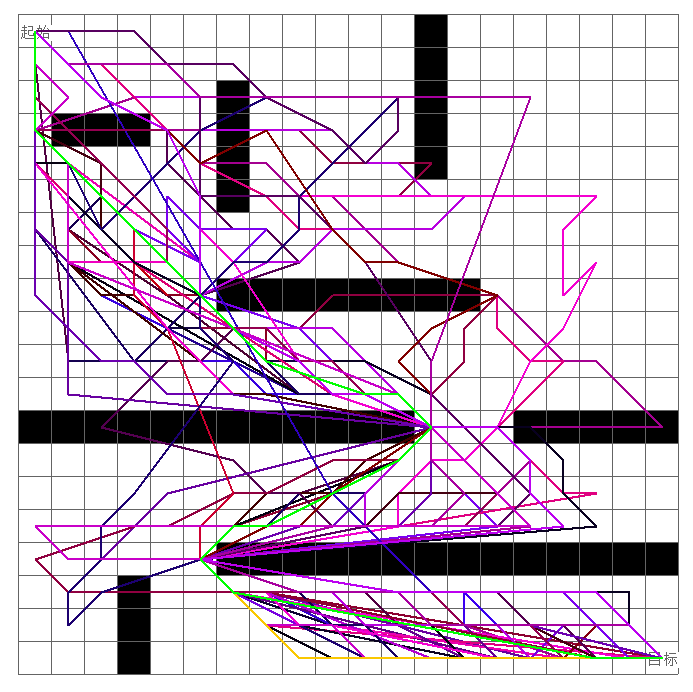
\includegraphics[width=1.5in]{images/200caea.png}
    }
    \end{center}
    \caption{Running screenshots at the $200th$}
\end{figure}
\begin{figure}[htb]
    \begin{center}
    \subfigure[NSGA-II]
    {
        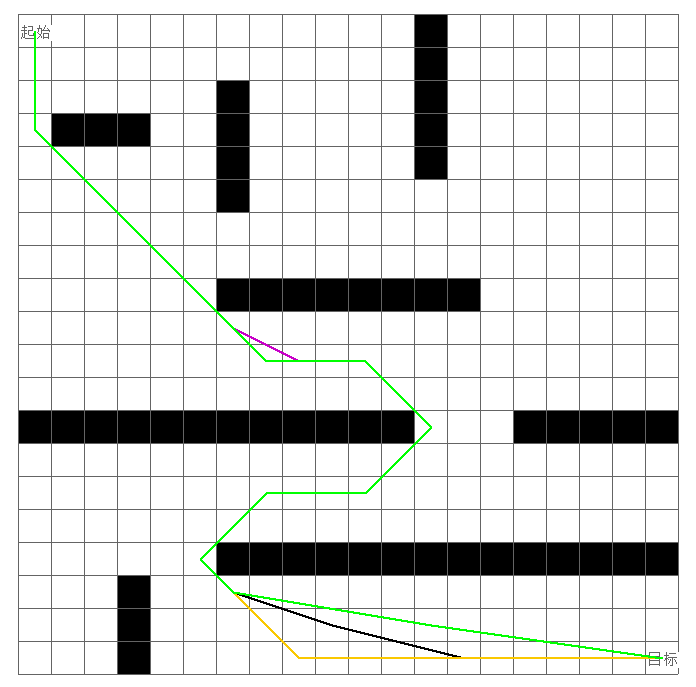
\includegraphics[width=1.5in]{images/500nsga.png}
    }
    \subfigure[MOEA/D]
    {
        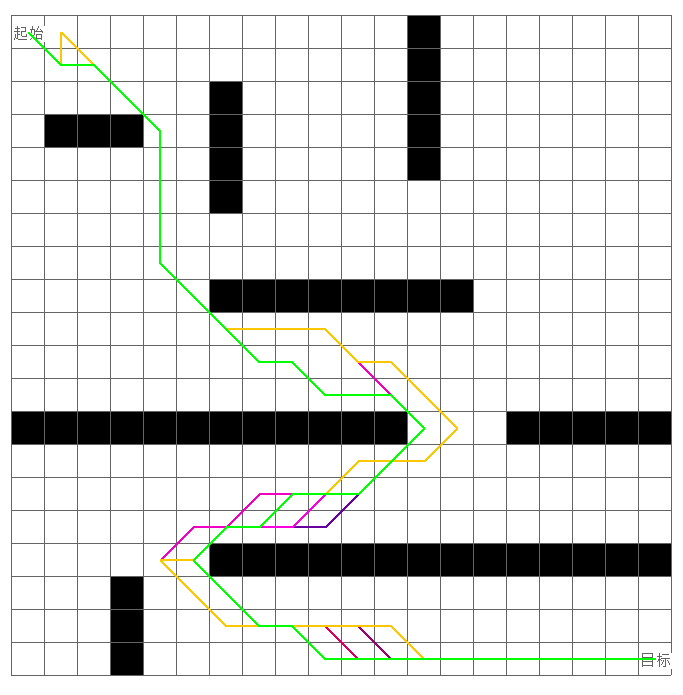
\includegraphics[width=1.5in]{images/500moead.png}
    }
    \subfigure[CAEA]
    {
        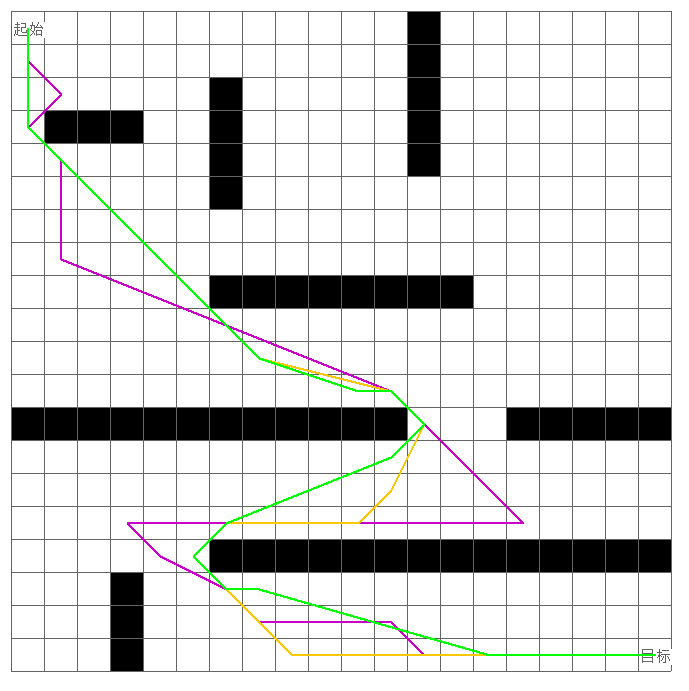
\includegraphics[width=1.5in]{images/500caea.png}
    }
    \end{center}
    \caption{Running screenshots at the $500th$}
\end{figure}
\begin{flushleft}
At $500th$, regardless of some paths caused by mutation, most the paths are converged.
From $100th$ to $200th$, we can clearly see that the diversity of three of CAEA is better than the other two,
and MOEA/D is better than NSGA-II.
\end{flushleft}

\subsubsection{Test 2: Population}
Test 2 is testing the interaction of population size and results.
Under the condition of crossover rate = $0.9$, mutation rate = $0.1$ and generation = $500$,
we collected three sets of results for each algorithm. The variable is the size of population:
$40$, $100$, $200$.\\
\\
This is the data table:
\clearpage
\begin{table}[htb]
  \centering
    \begin{tabular}{|l|l|c|c|c|}
    \hline
    \multicolumn{2}{|c|}{Populations size:}& 40 & 100 & 200\\
    \hline
    \multirow{3}{*}{NSGA-II}& Length & 0.286 & 0.286 & 0.328\\
                            & Smoothness & 0.105 & 0.143 & 0.139\\
                            & Security & 0.430 & 0.399 & 0.361\\
    \hline
    \multirow{3}{*}{MOEA/D} & Length & 0.378 & 0.332 & 0.298\\
                            & Smoothness & 0.189 & 0.192 & 0.200\\
                            & Security & 0.382 & 0.360 & 0.333\\
    \hline
    \multirow{3}{*}{CAEA}   & Length & 0.353 & 0.351 & 0.350\\
                            & Smoothness & 0.156 & 0.151 & 0.171\\
                            & Security & 0.388 & 0.344 & 0.370\\
    \hline
    \end{tabular}
  \caption{Data of different population size.}
\end{table}
\begin{figure}[htb]
    \begin{center}
    \subfigure[NSGA-II]
    {
        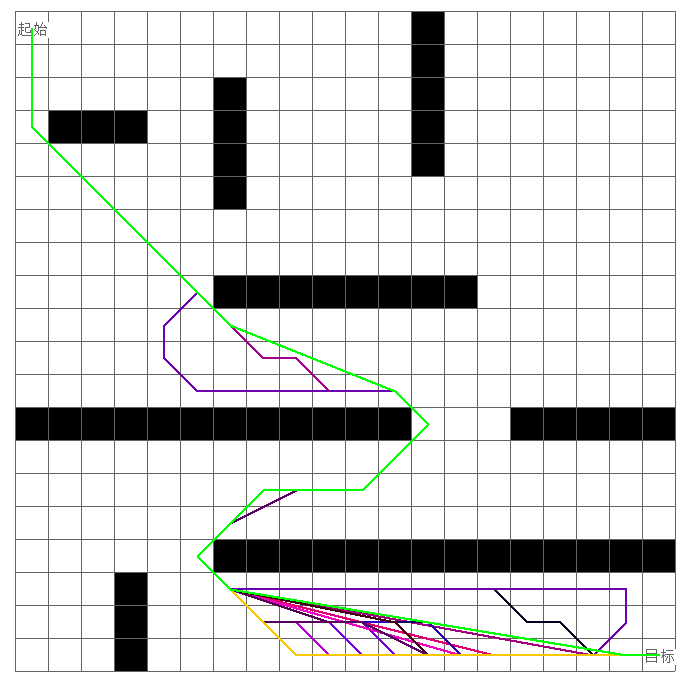
\includegraphics[width=1.5in]{images/40pcaea.png}
    }
    \subfigure[MOEA/D]
    {
        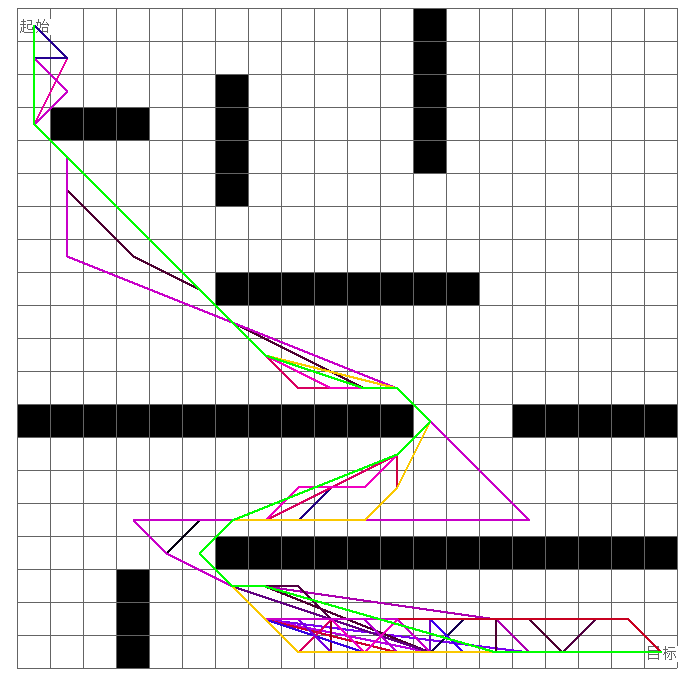
\includegraphics[width=1.5in]{images/100pcaea.png}
    }
    \subfigure[CAEA]
    {
        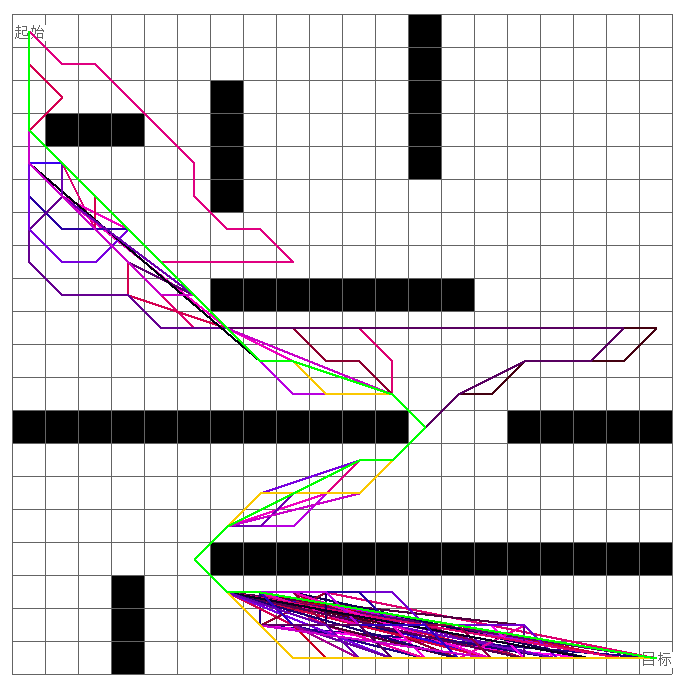
\includegraphics[width=1.5in]{images/200pcaea.png}
    }
    \end{center}
    \caption{CAEA under different population size}
\end{figure}

\begin{flushleft}
Because of the large generation and the high crossover rate, the influence of population size is not very considerable.
On the other hand, the larger the population is, the more diversity it has. The population of $40$ is the lowest feasible
size.
\end{flushleft}

\subsubsection{Test 3: Crossover Rate}
Test 3 is about the connection between crossover rate and results.
Crossover is the major operation of reproduction, so the rate should not be too low.
Other parameters: $mutation\ rate\ =\ 0.1$; $population\ size\ =\ 100$; $generation\ =\ 500$.
In this test, we used the rate of $0.4$, $0.65$ and $0.9$, and the data is as shown below:
\clearpage
\begin{table}[htb]
  \centering
    \begin{tabular}{|l|l|c|c|c|}
    \hline
    \multicolumn{2}{|c|}{Crossover rate:}& 0.9 & 0.65 & 0.4\\
    \hline
    \multirow{3}{*}{NSGA-II}& Length & 0.286 & 0.315 & 0.369\\
                            & Smoothness & 0.143 & 0.762 & 0.706\\
                            & Security & 0.399 & 0.424 & 0.372\\
    \hline
    \multirow{3}{*}{MOEA/D} & Length & 0.370 & 0.373 & 0.367\\
                            & Smoothness & 0.140 & 0.111 & 0.115\\
                            & Security & 0.351 & 0.395 & 0.368\\
    \hline
    \multirow{3}{*}{CAEA}   & Length & 0.351 & 0.355 & 0.355\\
                            & Smoothness & 0.151 & 0.194 & 0.192\\
                            & Security & 0.344 & 0.364 & 0.378\\
    \hline
    \end{tabular}
  \caption{Data of different crossover rate.}
\end{table}
\begin{flushleft}
This table shows us that under the condition of $0.4$ and $0.65$ crossover rate, NSGA-II generated results which are much worse than under $0.9$ crossover rate.
\end{flushleft}

\begin{figure}[htb]
    \begin{center}
    \subfigure[NSGA-II]
    {
        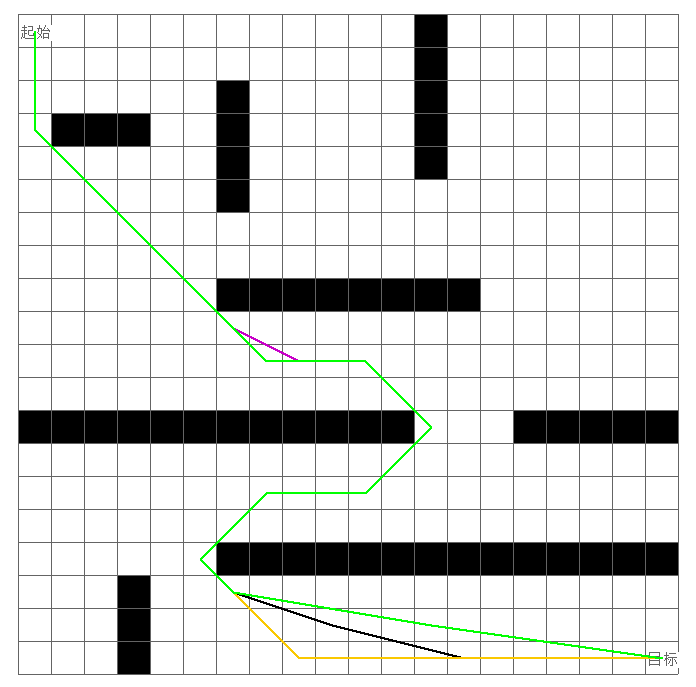
\includegraphics[width=1.5in]{images/500nsga.png}
    }
    \subfigure[MOEA/D]
    {
        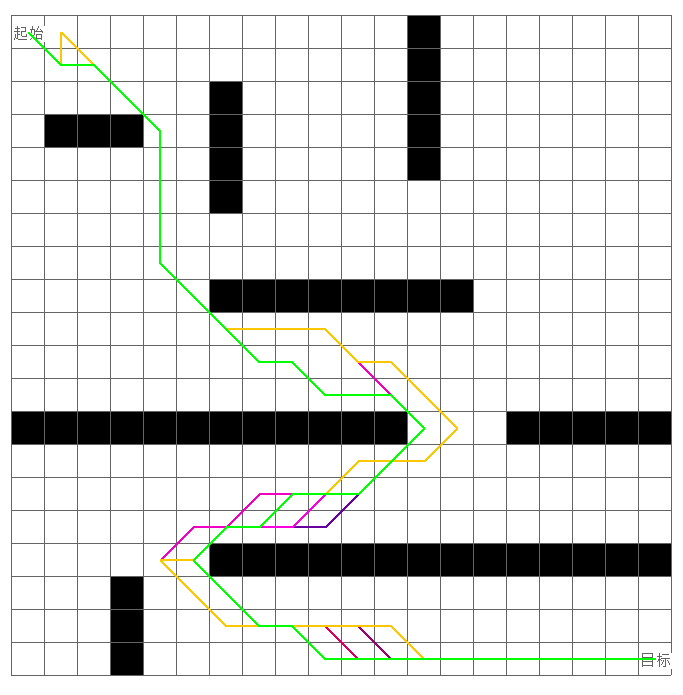
\includegraphics[width=1.5in]{images/500moead.png}
    }
    \subfigure[CAEA]
    {
        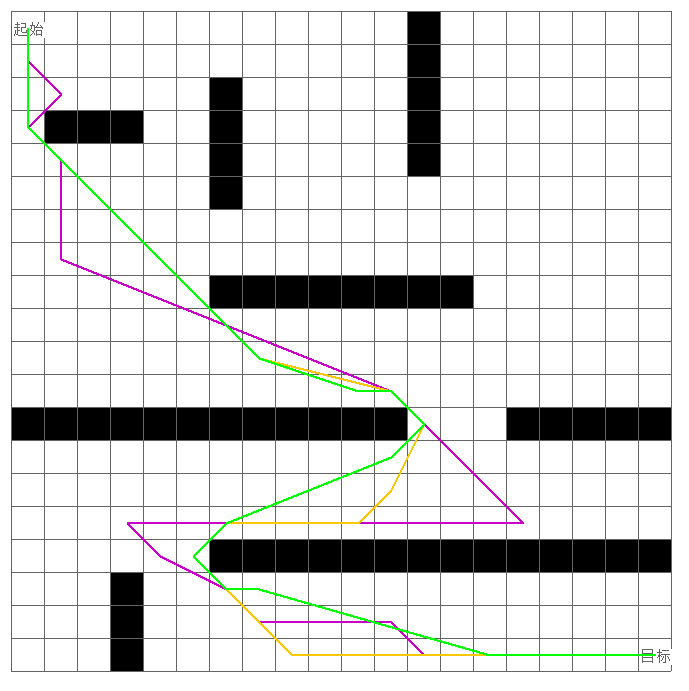
\includegraphics[width=1.5in]{images/500caea.png}
    }
    \end{center}
    \caption{Crossover rate: 0.9}\label{fig:9cr}
\end{figure}
\begin{flushleft}
In Figure \ref{fig:9cr} three of them can generate feasible results.
However, if the rate is lower, we can see some changes as shown in Figure \ref{fig:65rc} and Figure \ref{fig:4rc}.
In NSGA-II, the individuals with higher diversity is selected by $crowding distance$ method. But with lower crossover rate,
these individuals are hard to preserve.
\end{flushleft}
\clearpage
\begin{figure}[htb]
    \begin{center}
    \subfigure[NSGA-II]
    {
        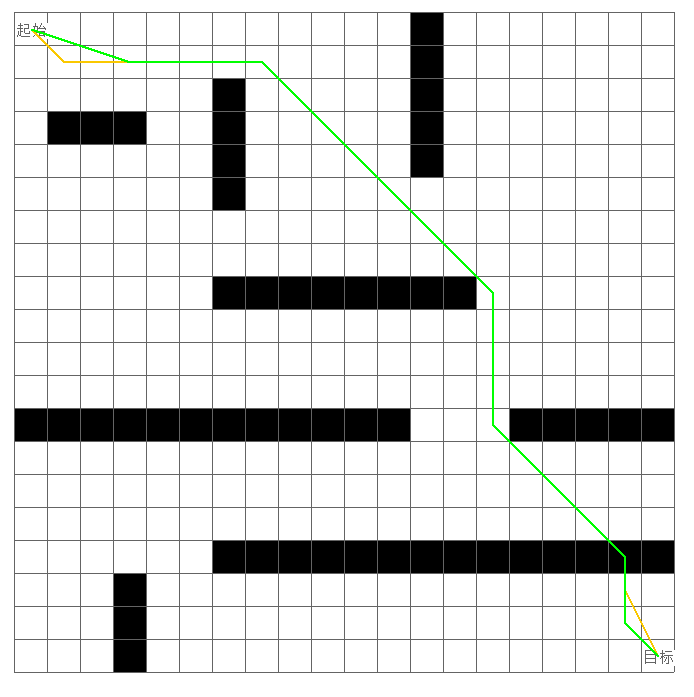
\includegraphics[width=1.5in]{images/65nsga.png}
    }
    \subfigure[MOEA/D]
    {
        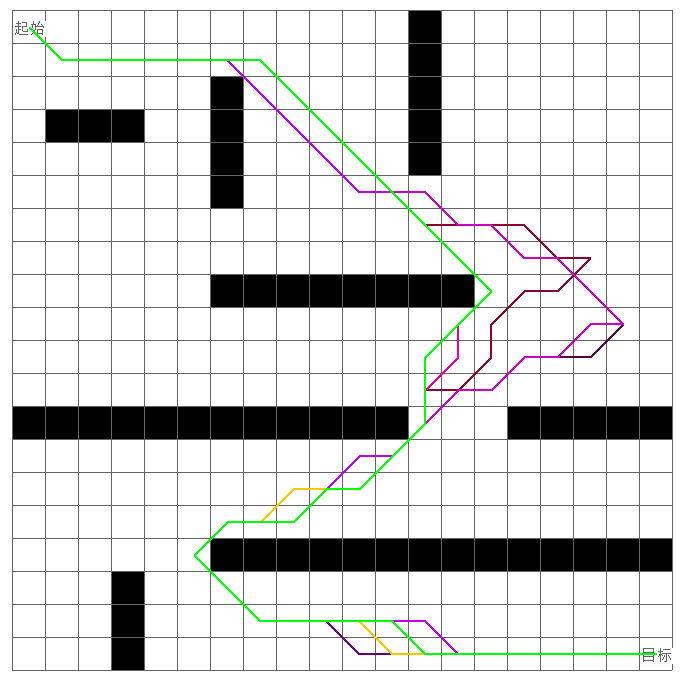
\includegraphics[width=1.5in]{images/65moead.png}
    }
    \subfigure[CAEA]
    {
        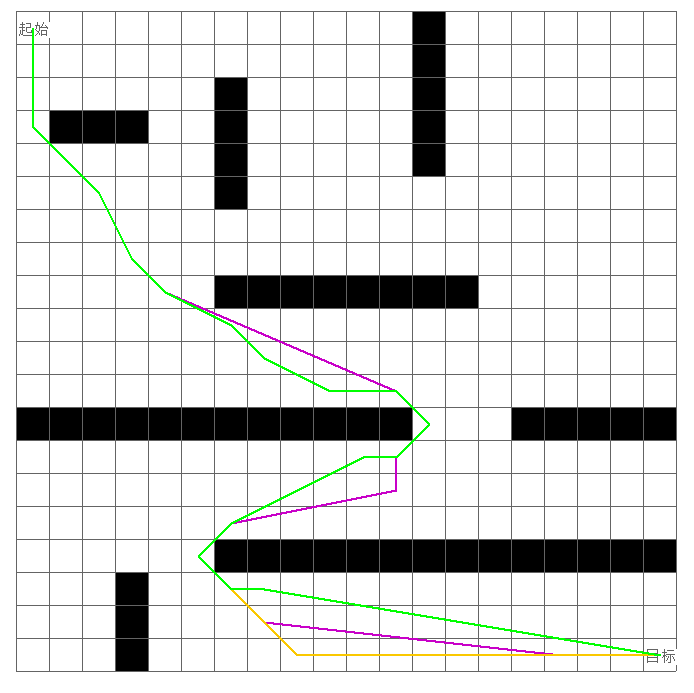
\includegraphics[width=1.5in]{images/65caea.png}
    }
    \end{center}
    \caption{Crossover rate: 0.65}\label{fig:65rc}
\end{figure}
\begin{figure}[htb]
    \begin{center}
    \subfigure[NSGA-II]
    {
        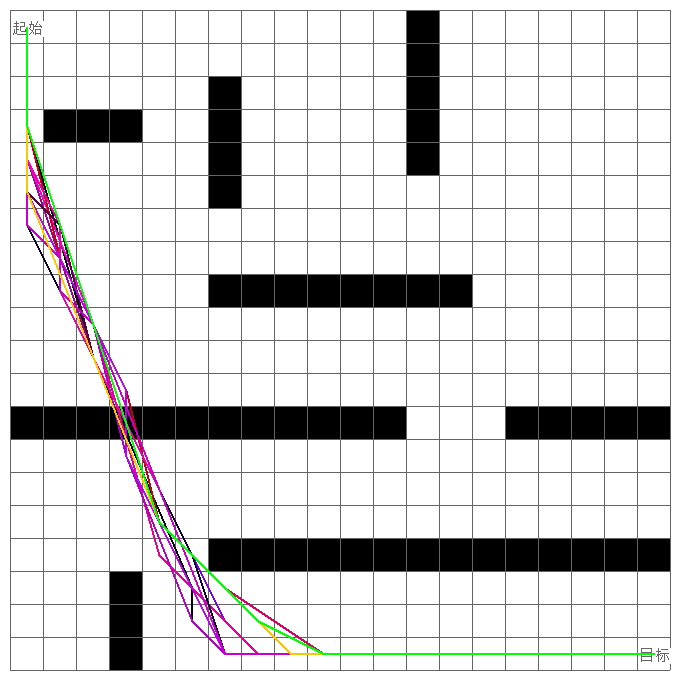
\includegraphics[width=1.5in]{images/4nsga.png}
    }
    \subfigure[MOEA/D]
    {
        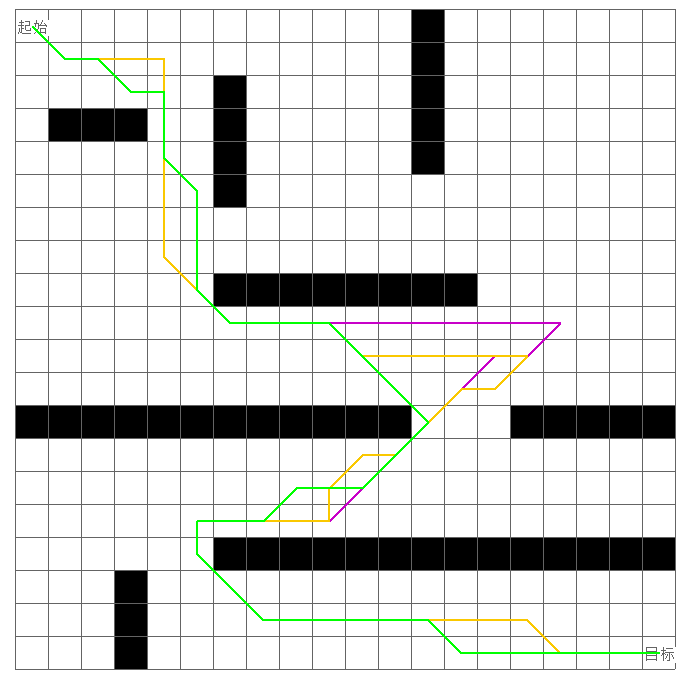
\includegraphics[width=1.5in]{images/4moead.png}
    }
    \subfigure[CAEA]
    {
        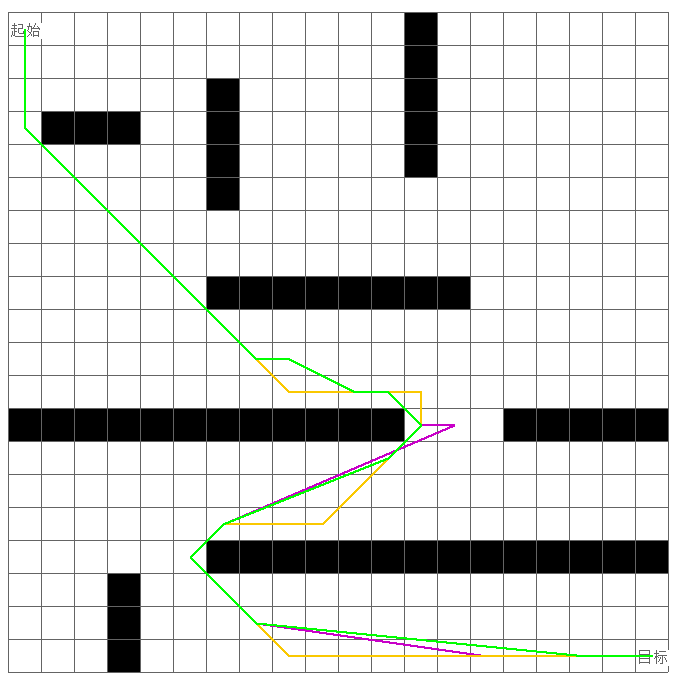
\includegraphics[width=1.5in]{images/4caea.png}
    }
    \end{center}
    \caption{Crossover rate: 0.4}\label{fig:4rc}
\end{figure}
\noindent These running screenshots illustrate that the diversity preservation of NSGA-II has a closely link to the crossover rate.
In some extreme condition, if the crossover rate is not high enough, the diversity preserving efficiency of NSGA-II will
decrease, which might lead to some bad solutions. In contrast, MOEA/D and CAEA can still generate feasible results.


%----------------------------------------------------------------------------------------
%----------------------------------------------------------------------------------------
\subsection{Section Conclusion}
In this section, we introduce the environment of this experiment and the three tests we did by data table and screenshots.
It was shown in the before that comparison of three algorithm in data and figures. This is a direct way to show the difference
of three algorithm we used.
\newpage

%----------------------------------------------------------------------------------------
%	Results and Conclusions
%----------------------------------------------------------------------------------------

\section{Conclusion}
This article introduced the renowned \emph{Evolutionary Algorithms}:
NSGA-II and MOEA/D, and a very new EA based on decomposition: CAEA.
In addition, we analysed that how to use EAs to solve a very old and classic problem,
Robot Path Planning, by changing it to a \emph{Multiobjective Optimization Problem}.
Finally, we did some tests about this problem by using these three EAs, and collected
data and then made some conclusions.\\
\\
NSGA-II, MOEA/D and CAEA, all these three EAs are very suitable for solving Robot Path Planning problem. NSGA-II is a very stable EA.
As for this problem, it can generate a set of solutions with relatively high feasibility in a single run. Furthermore, it can optimize the whole
population and make them close to the Pareto Front. Nevertheless, the efficiency of NSGA-II and its diversity of solution are not very high.\\
\\
MOEA/D is an EA based on decomposition, which means it has a very fast
performance speed. The theoretical basis and the test results of MOEA/D
show that this is a revolutionary EA.\\
\\
CAEA is proposed by my tutor, professor YING, which also is based on decomposition.
It has been proved that CAEA has very low time-consuming compared to NSGA-II and CAEA.
This means that CAEA can run faster than NSGA-II and MOEA/D. In this article,
we can conclude that the diversity of the solutions of CAEA is higher than NSGA-II
and MOEA/D. Diversity is an important indicator of an EA, and this shows the potential
of CAEA.CAEA can only solve biobjective optimization problem by now. The research for tri-
and multi-objective optimization problem is still ongoing. \\
\\
Finally, my team and I truly appreciate professor YING and his help for this research project.
\newpage

%----------------------------------------------------------------------------------------
%	BIBLIOGRAPHY
%----------------------------------------------------------------------------------------

\bibliographystyle{unsrt}
%
\bibliography{pathplanning_report}

%----------------------------------------------------------------------------------------


\end{document}
